\documentclass[listof=totoc]{scrartcl}
\usepackage[utf8]{inputenc}
\usepackage[activate={true,nocompatibility},final,tracking=true,kerning=true,spacing=true,factor=1100,stretch=10,shrink=10]{microtype}
\usepackage[english]{babel}
\usepackage{csquotes}
\usepackage{hyperref}
\usepackage[style=ieee, autocite=inline, backend=biber]{biblatex}
\usepackage[binary-units=true]{siunitx}
\usepackage{todonotes}
\usepackage{parskip}
\usepackage{pgfplots}
\usepackage[nomarkers,figuresonly,nolists,noheads]{endfloat}

\microtypecontext{spacing=nonfrench}
\pgfplotsset{compat=1.15}
\addbibresource{references.bib}

\renewcommand{\efloatseparator}{\mbox{}}

\subject{BUSAN 100G: Digital Information Literacy}
\title{Stack Overflow Visualisation \& Analysis}
\author{Jackson Chadfield}
\date{\today}

\begin{document}

\maketitle
\listoffigures

\section{Topic}
I have decided to analyse the annual Stack Overflow developer survey\cite{dataset}.
As a professional programmer, this data is fascinating and gives me insight on upcoming technologies to learn. The world of technology is constantly changing and it is important for me to be aware of current best practices.

\section{Source}
Stack Overflow is a knowledge sharing site for programmers and is one of the first places to check when you have a problem related to programming.

Stack Overflow surveys developers using their site annually. It is one of the best sources of data for current trends due to the site being used by so many developers all over the world. Stack Overflow released the anonymous dataset under the Open Database License.

The data is contained in a simple tabular CSV file with 85 columns. The description of what each column measures can be found in the schema file published alongside the dataset. In total, the dataset contains \num{88883} rows. The data is for a single year, so trends cannot be visualised without including previous datasets.

Unfortunately, since GitHub maintains a file size limit of \SI{100}{\mega\byte} and the dataset approaches \SI{200}{\mega\byte}, I cannot store it in my version control. It is, however, easily accessible online.

\section{Analysis \& Visualisation}
All visualisations were created using Tableau. Ages were rounded to the nearest whole number to keep consistent measurement. Some columns used multiple values in a single cell, which Tableau does not support. To work around this, I developed a script which creates correctly formatted auxiliary files. This file is available with the rest of my files\cite{repo}. Where a column has multiple values per cell, each respondent may have more than one response. This means that the sum of values visualisations shown in \autoref{subsection:topicspecific} may exceed the number of respondents.

\subsection{Demographic}
\begin{figure}
    \centering
    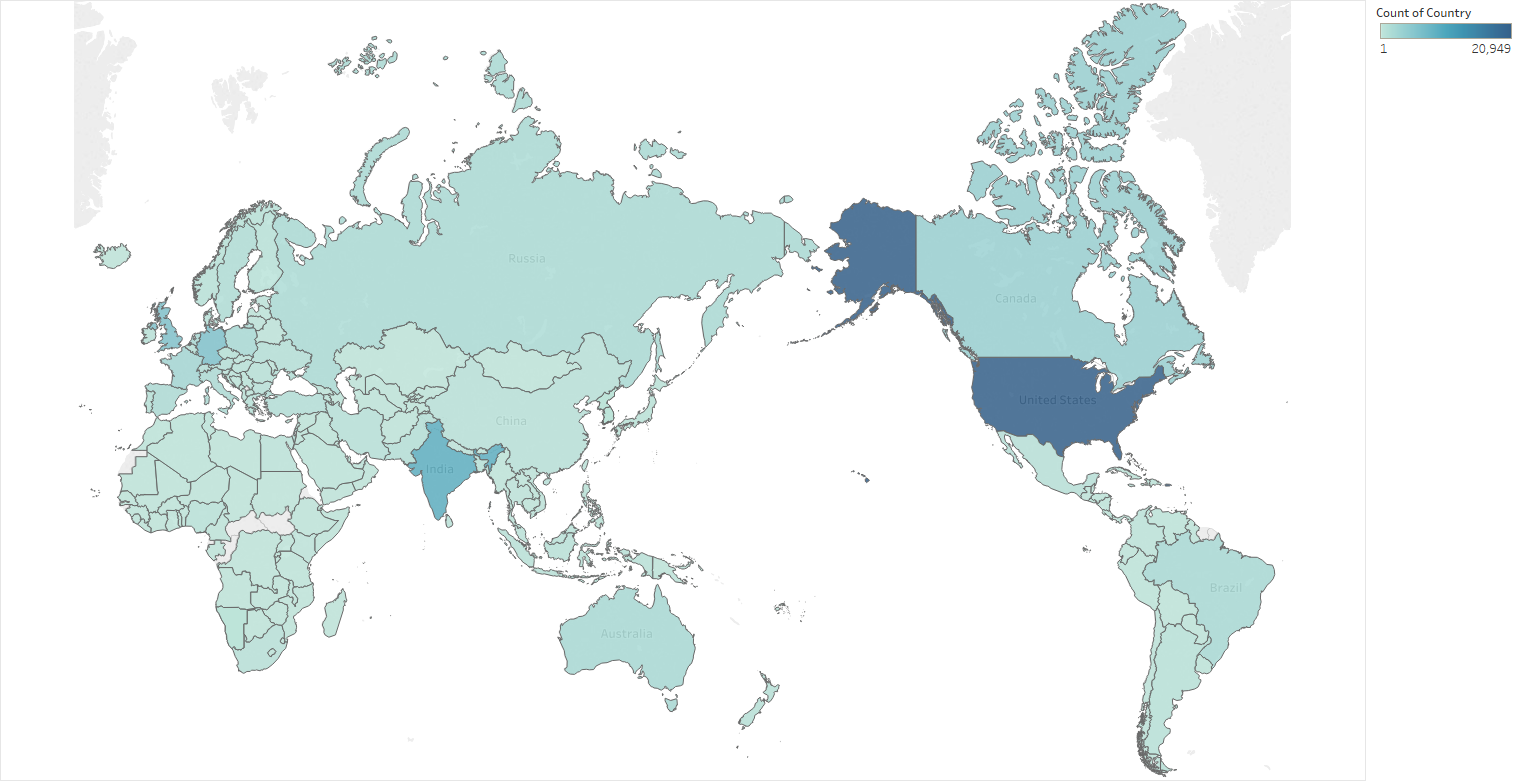
\includegraphics[width=\textwidth]{Documentation/images/map.png}
    \caption{Responses per Country}
    \label{fig:country_responses}
\end{figure}
\begin{figure}
    \centering
    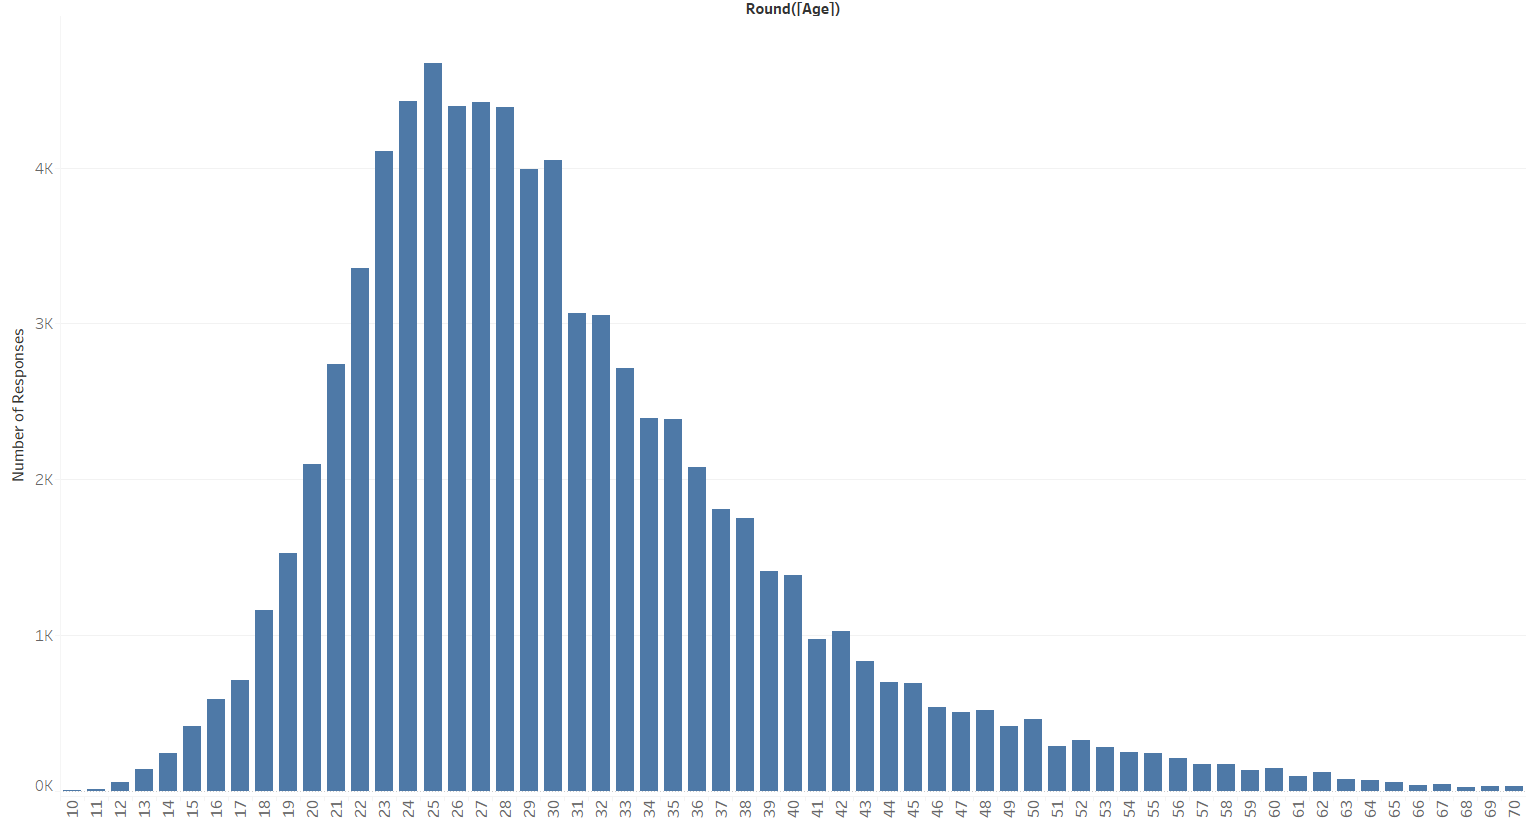
\includegraphics[width=\textwidth]{Documentation/images/age.png}
    \caption{Responses per Age}
    \label{fig:age_responses}
\end{figure}
\begin{figure}
    \centering
    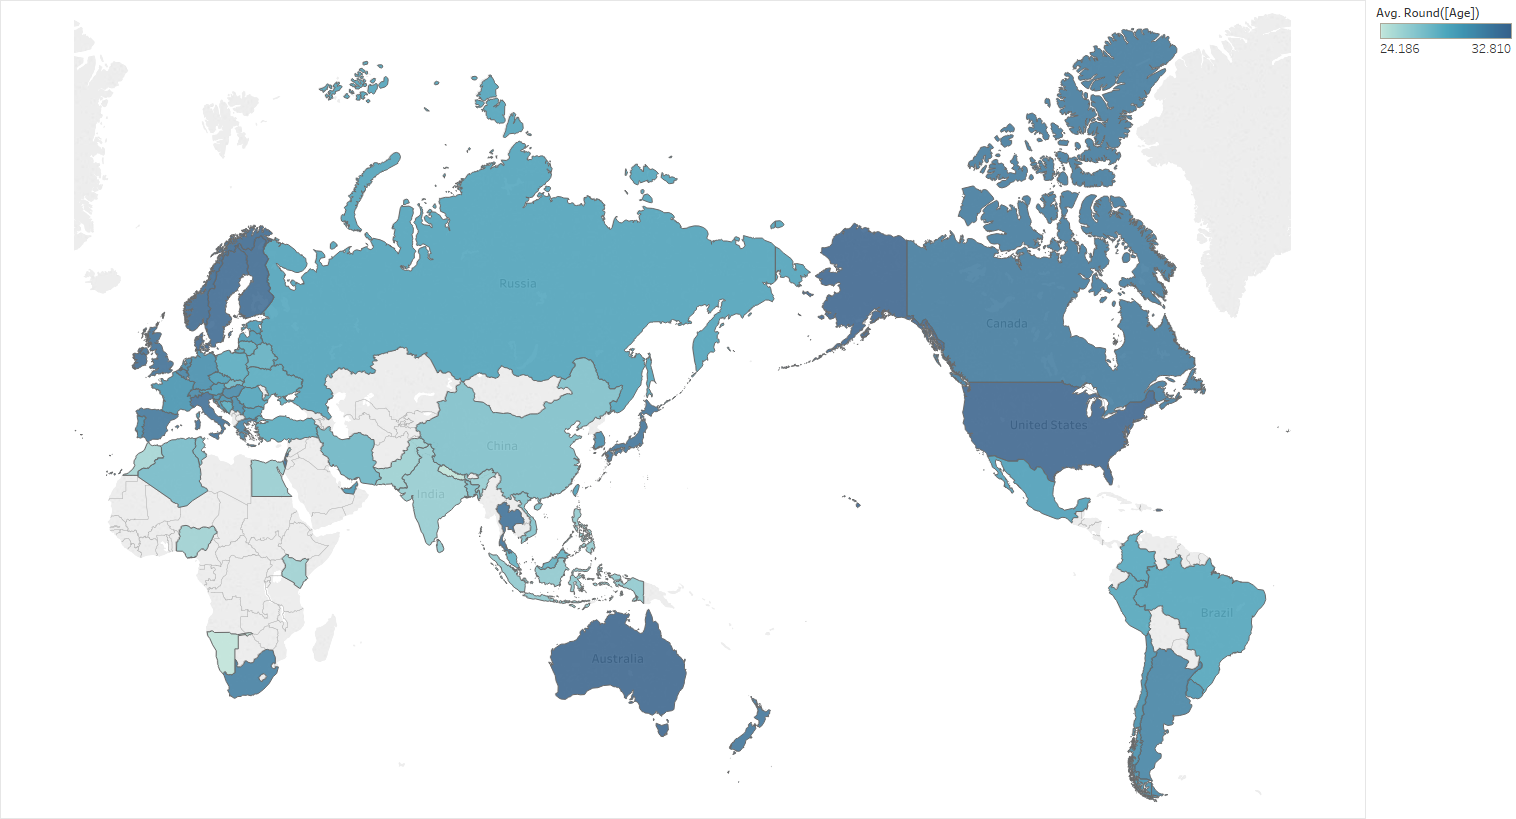
\includegraphics[width=\textwidth]{Documentation/images/average_age.png}
    \caption{Average Age per Country}
    \label{fig:average_age}
\end{figure}
As shown in \autoref{fig:country_responses}, the majority of responses originate from the United States. The second highest country, India, has less than half of the United States total responses. Together they form roughly \(\frac{1}{3}\) of the responses. In comparison, New Zealand totals \num{524} responses (~0.6\% of the total responses). The bias towards the United States may be due to Stack Overflow being an American website with more content for English speakers.

The age of respondents (\autoref{fig:age_responses}) is a normal distribution. With the majority being within \numrange{20}{40} years old. I was also curious about the average age in each country. This visualisation can be seen in \autoref{fig:average_age}. I only included countries with 100 or more responses, so that results would not be skewed by countries with a singular response that is not representative of the population.

\subsection{Topic Specific}
\label{subsection:topicspecific}
\begin{figure}
    \centering
    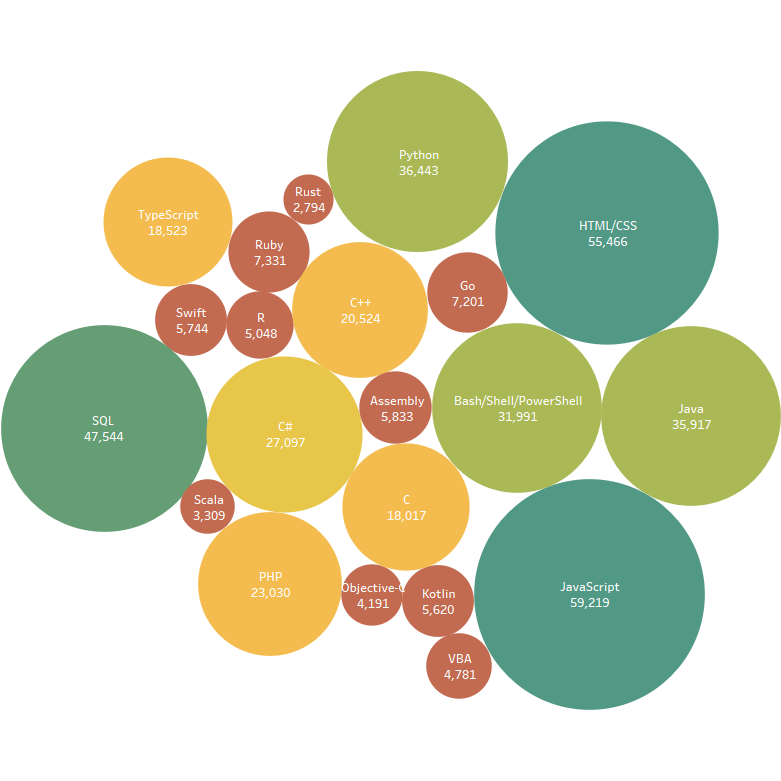
\includegraphics[width=\textwidth]{Documentation/images/languages.png}
    \caption{Usage of Programming Languages for Work}
    \label{fig:languages}
\end{figure}
\begin{figure}
    \centering
    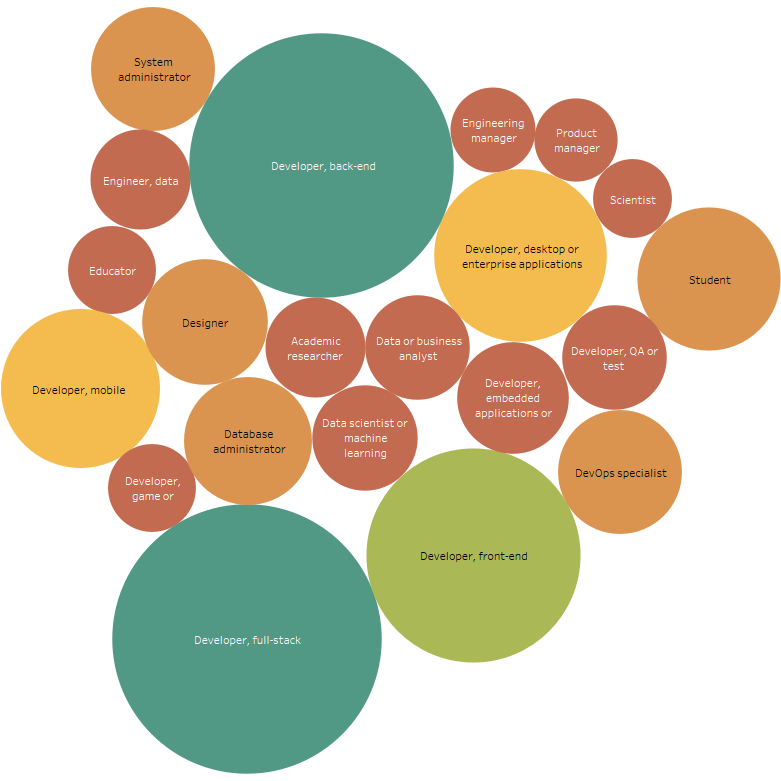
\includegraphics[width=\textwidth]{Documentation/images/types.png}
    \caption{Developer Roles of Respondents}
    \label{fig:devtypes}
\end{figure}
One of the most crucial aspects of programming is the language used. \autoref{fig:languages} shows the languages that respondents said that they used for their work. JavaScript \& HTML/CSS hold the top spot, with 27\% of all respondents working with them. These three languages are generally paired together when being used to create a Front-End web application. This visualisation indicates that the majority of professional programmers have a role that involves managing web content. This hypothesis is backed by \autoref{fig:devtypes}, where the top 3 roles are related to managing some form of internet content.

One of the more surprising results of the survey is that more jobs use Python rather than Java. Java has historically been regarded as the default language for professional applications. This can (crudely) be seen on Google trends\cite{TrendsPythonVsJava}.

\section{Report Management}
This document was written in \LaTeX{}\autocite{LaTeX}. Primarily through the online service Overleaf, but also occasionally compiled manually.

I use the distributed version control system git\autocite{git} to keep versions of my source code available (this includes both this document and any code used). Since I am the sole contributor to this project and it is relatively small I used a simple linear master branch. I use GitHub as a centralised store for my repository. All versions of my source can be accessed online\autocite{repo}

I originally managed my references with Zotero, but found many problems with using it with Bib-\LaTeX{}. The citation keys it generated were messy and many fields were incorrectly populated. I tried Mendeley as an alternative but ultimately found it much easier to write the database entries manually. This gives me similar benefits to using

I use Bib-\LaTeX{} as my back-end for my referencing, which will automatically add a reference list and citations where needed.

This tool-set allows me to access my work from any location: either from overleaf, or by cloning my repository and manually compiling my document. It also gives freedom for my work flow to be integrated directly into this document. For example, if I add or change a reference, the document will automatically update and insert it in any relevant locations.

\printbibliography

\end{document}
